\begin{tikzpicture}	
	\draw[->, very thick, red] (22:8cm) arc[radius=1, start angle=140, end angle=40] node[above, red] at (8.3, 3.3) {$z \rightarrowtail w = f(z)$} node at (8.3, 2.3) {$f(z) = a \cdot z + b$};
	
	\begin{tikzpicture}
	\begin{axis}[
		axis lines=middle,
		axis equal,
		xmin=-4,
		xmax=4,
		ymin=-4,
		ymax=4,
		xlabel=$z_1$,
		ylabel=$z_2$,
		xticklabels={,,},
		yticklabels={,,}
	]
		\addplot[-, yellow, ultra thick] coordinates {(-2.5, 2) (2.5, 2)};
		\addplot[-, black!70!green, ultra thick] coordinates {(-2.5, 1) (2.5, 1)};
		\addplot[-, cyan, ultra thick] coordinates {(-2.5, 0) (2.5, 0)};
		\addplot[-, black!50!blue, ultra thick] coordinates {(-2.5, -1) (2.5, -1)};
		\addplot[-, blue, ultra thick] coordinates {(-2.5, -2) (2.5, -2)};
		
		\addplot[-, purple, ultra thick] coordinates {(-2, -2.5) (-2, 2.5)};
		\addplot[-, pink, ultra thick] coordinates {(-1, -2.5) (-1, 2.5)};
		\addplot[-, black!50!red, ultra thick] coordinates {(0, -2.5) (0, 2.5)};
		\addplot[-, orange, ultra thick] coordinates {(1, -2.5) (1, 2.5)};
		\addplot[-, red, ultra thick] coordinates {(2, -2.5) (2, 2.5)};
	\end{axis}
\end{tikzpicture}\hspace{2.7cm}%
	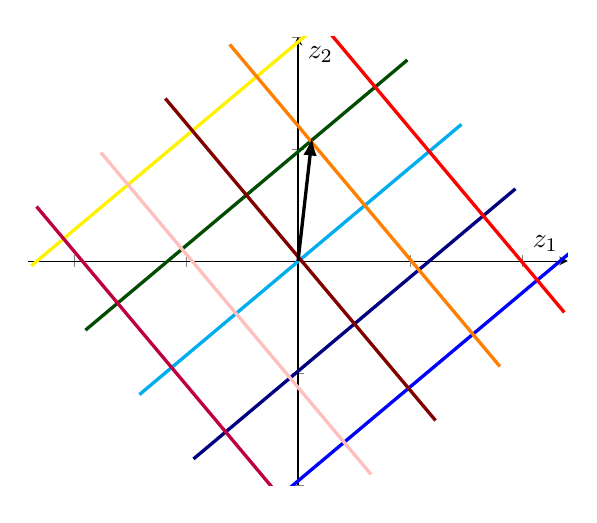
\begin{tikzpicture}
	\begin{axis}[
		axis lines=middle,
		axis equal,
		xmin=-4,
		xmax=4,
		ymin=-4,
		ymax=4,
		xlabel=$z_1$,
		ylabel=$z_2$,
		xticklabels={,,},
		yticklabels={,,}
	]
		\addplot[-, yellow, very thick, rotate=40, xshift=1.2cm, yshift=-2.5cm] coordinates {(-3.75, 3) (3.75, 3)};
		\addplot[-, black!70!green, very thick, rotate=40, xshift=1.2cm, yshift=-2.5cm] coordinates {(-3.75, 1.5) (3.75, 1.5)};
		\addplot[-, cyan, very thick, rotate=40, xshift=1.2cm, yshift=-2.5cm] coordinates {(-3.75, 0) (3.75, 0)};
		\addplot[-, black!50!blue, very thick, rotate=40, xshift=1.2cm, yshift=-2.5cm] coordinates {(-3.75, -1.5) (3.75, -1.5)};
		\addplot[-, blue, very thick, rotate=40, xshift=1.2cm, yshift=-2.5cm] coordinates {(-3.75, -3) (3.75, -3)};
		
		\addplot[-, purple, very thick, rotate=40, xshift=1.2cm, yshift=-2.5cm] coordinates {(-3, -3.75) (-3, 3.75)};
		\addplot[-, pink, very thick, rotate=40, xshift=1.2cm, yshift=-2.5cm] coordinates {(-1.5, -3.75) (-1.5, 3.75)};
		\addplot[-, black!50!red, very thick, rotate=40, xshift=1.2cm, yshift=-2.5cm] coordinates {(0, -3.75) (0, 3.75)};
		\addplot[-, orange, very thick, rotate=40, xshift=1.2cm, yshift=-2.5cm] coordinates {(1.5, -3.75) (1.5, 3.75)};
		\addplot[-, red, very thick, rotate=40, xshift=1.2cm, yshift=-2.5cm] coordinates {(3, -3.75) (3, 3.75)};
		
		\addplot[-latex, very thick] coordinates {(0, 0) (0.25, 2.2)};
	\end{axis}
\end{tikzpicture}
\end{tikzpicture}